\section{PID}
\begin{center}
 	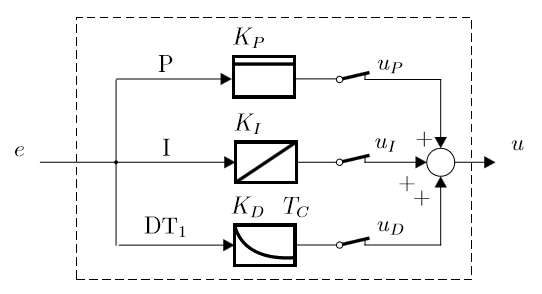
\includegraphics[width=\columnwidth]{Images/pid}
\end{center}

Die UTF bei einem realen PID-Regeler:
\[
G_{PID}(j\omega) = K_P + \frac{K_I}{j\omega} + K_D\frac{j\omega}{1+i\omega T_C}
\]

\subsection{Regler Parameter}
\subsubsection{PN Kürzung}
Diese Technik beruht darauf, dass ein LZI-Modell verliegt. Zudem müssen alle Pole in der Linken Halbebene sein d.h. wenn sie negative Realteile haben.

\subsubsection{Empirische Einstellregeler}
Ein erster Regler, welcher nicht optimal ist, kann zB mit ZN oder CHR gefunden werden. Dabei wird eine Schrittantwort aufgezeichnet und and Wendepunkt $Q$ eine Tangente angelegt. Damit ergeben sich $T_u$ und $T_g$. Diese können auch zu beurteilung, wie gut ein Regler funktioniert verwendet werden. \script{162}

\subsubsection{Optimierung}
Für verschiedene Parameter werden Experimente durchgeführt, bei denen der relevante Fehler $e$ und Stellsignal $u$ aufgezeichnet werden. Zur Beurteilung wird nun das minimum von $J(k_1, \dots, k_m) ) \int_{0}^{T_{end}}e(t)^2dt$ berechnet.
\script{165}

\subsection{Wind-up}
Das Wind-up Problem kann auftreten, wenn drei Voraussetzungen zusammenfallen \script{170}:
\begin{enumerate}[nosep]
	\item Der Regler beinhaltet einen I-Anteil. d.h. einen offenen Integrator
	\item Das Stellglied ist limitiert. d.h. enthält eine Sättigung
	\item e(t) über eine längere Zeit $\neq$ 0
\end{enumerate}

\subsection{Störgrössenaufschaltung}
Statt auf Störungen in einem Regler zu reagieren, wird versucht diese mit einer SGA (Störgrössenaufschaltung, was dem Inversen-Regler entspricht) vor dem Regler zu addieren, dadurch werden Störungen minimiert, was zu einem schnelleren Regler führt. \script{171}

\begin{center}
	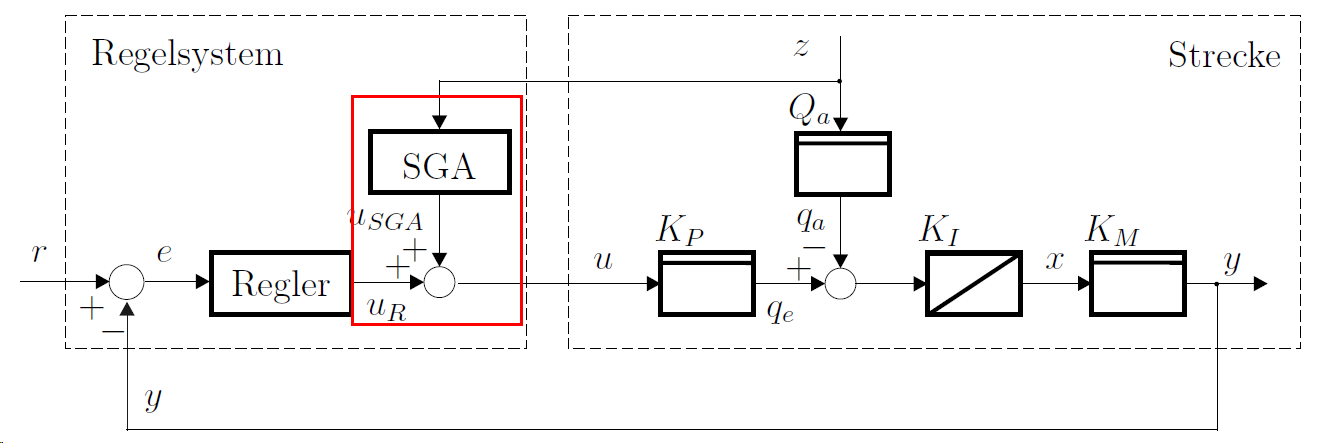
\includegraphics[width=0.8\columnwidth]{Images/sga1}
\end{center}

\subsection{Implementierung von Reglern}
\script{175}